\documentclass[border=2pt]{standalone}
\usepackage{pgfplots}
\pgfplotsset{compat=1.18}
\begin{document}
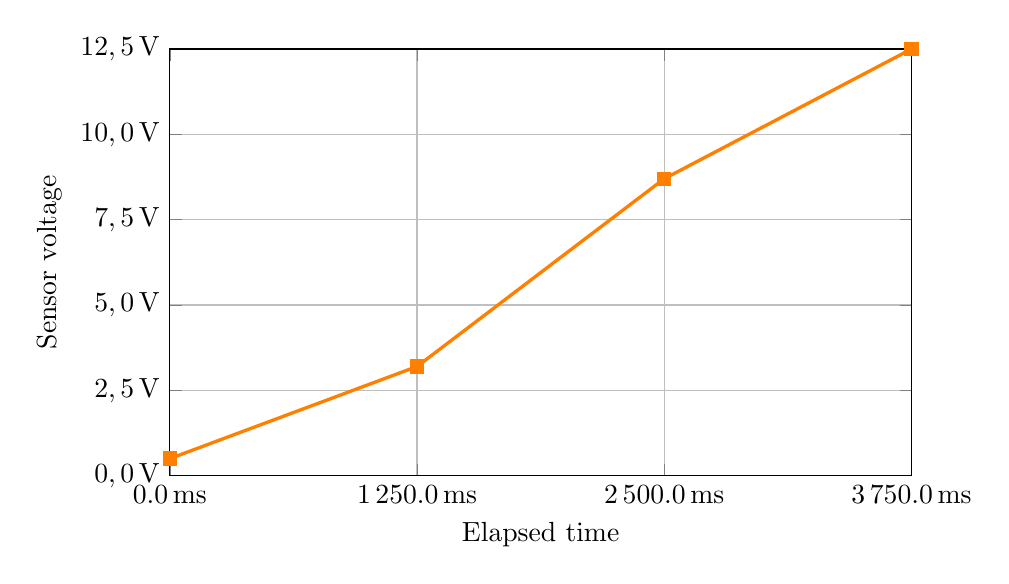
\begin{tikzpicture}
  \begin{axis}[
    width=11cm,
    height=7cm,
    xmin=0,
    xmax=3750,
    ymin=0,
    ymax=12.5,
    xtick={0,1250,2500,3750},
    ytick={0,2.5,5,7.5,10,12.5},
    xticklabel={$\pgfmathprintnumber[fixed,fixed zerofill,precision=1,1000 sep={\,}]{\tick}\,\mathrm{ms}$},
    yticklabel={$\pgfmathprintnumber[fixed,fixed zerofill,precision=1,set decimal separator={,}]{\tick}\,\mathrm{V}$},
    grid=major,
    xlabel={Elapsed time},
    ylabel={Sensor voltage}
  ]
    \addplot[orange,very thick,mark=square*] coordinates {
      (0,0.5) (1250,3.2) (2500,8.7) (3750,12.5)
    };
  \end{axis}
\end{tikzpicture}
\end{document}
